\documentclass[twocolumn]{article}

% Language setting
% Replace `english' with e.g. `spanish' to change the document language
\usepackage[spanish]{babel}

% Set page size and margins
% Replace `letterpaper' with`a4paper' for UK/EU standard size
\usepackage[letterpaper,top=2cm,bottom=2cm,left=2cm,right=2cm,marginparwidth=1.75cm]{geometry}

% Useful packages
\usepackage{amsmath}
\usepackage{graphicx}
\usepackage{hyperref}
\usepackage{apacite}

\title{Grafos}
\author{Barreiro Valdez Alejandro}

\begin{document}
\maketitle

%\tableofcontents
%\newpage

\section{Conceptos básicos}
Un grafo es una estructura de datos no lineal que está conformado por un conjunto de nodos o vértices y que son conectados por aristas o arcos. En los nodos se almacena algún dato y las aristas ayudan a relacionar esos nodos.

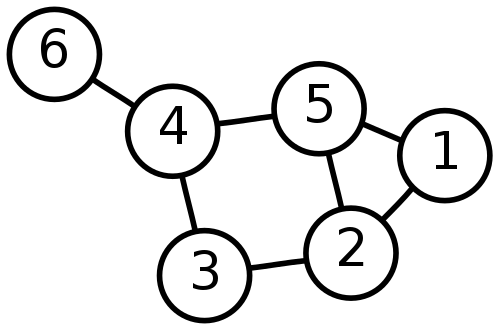
\includegraphics[width = .45\textwidth]{imagenes/grafo.png}

\subsection{Vértice}
En grafos, un vértice es cada uno de los nodos o de los elementos que conforman un grafo.
\subsection{Arista}
La arista entre dos vértices de un grafo es la conexión entre estos dos vértices.
\subsection{Grado}
El grado de un vértice es el número de aristas conectadas a un vértice.
\subsection{Adyacencia}
Se dice que dos vértices son adyacentes si hay una arista conectándolos.

\section{Clasificación de grafos}
\subsection{Grafos dirigidos}
También es conocido como dígrafo, las aristas de este tipo de grafo tienen una dirección. Esto quiere decir que la arista parte de un nodo para llegar a otro.
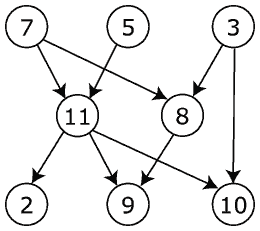
\includegraphics[width = .45\textwidth]{imagenes/dirigido.png}
\subsection{Grafos no dirigidos}
Un grafo donde todos las aristas son bidireccionales. Cuando se tienen dos vértices adyacentes en un grafo no dirigido, se puede ir de uno a otro sin importar de cuál se está partiendo.

\subsection{Grafo ponderado}
Los grafos ponderados son aquellos donde las aristas tienen un valor. Los valores que se asocian a la arista se llaman peso. Estos valores pueden representar un costo, una longitud, el peso o la velocidad.
\cite{upgrad}

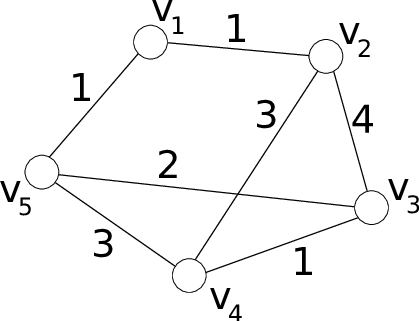
\includegraphics[width = .45\textwidth]{imagenes/ponderado.png}


\subsection{Grafo no ponderado}
Este tipo de grafos no tiene un valor asociado con las aristas. Todos los grafos son no ponderados hasta que se asocia algún valor con las aristas.

\section{Representación de grafos}
\subsection{Matriz de adyacencia}
Una matriz de adyacencia es una matriz cuadrada (nxn) donde se indican las relaciones de adyacencia entre nodos. Si existe una arista entre el vértice i y el vértice j se debe poner un número en la posición i,j de la matriz. Para los grafos no ponderados se utiliza un uno si existe la arista y un cero si no. Para los grafos ponderados se pone el valor del peso o cero en caso de que no exista la arista. En los grafos no dirigidos se obtiene como resultado una matriz simétrica porque se tienen relaciones bidireccionales.
La representación es fácil de implementar y de seguir. Para recorrer todos los vecinos de un nodo el proceso se vuelve tardado.


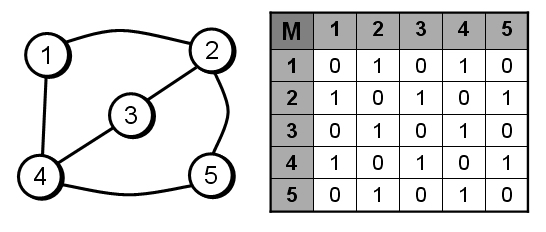
\includegraphics[width = .45\textwidth]{imagenes/Matriz_de_adyacencia.jpg}

\subsection{Matriz de incidencia}
Esta matriz se construye utilizando el número de vértices como el número de filas y el número de aristas como el número de columnas. La matriz se llena con los valores de 1, -1 y 0. Se utiliza 1 para aquellas aristas que salen del vértice. Se utiliza -1 para aquellas aristas que ingresan al vértice. Se utiliza 0 cuando la arista no tiene conexión con el vértice.
\cite{deepali}
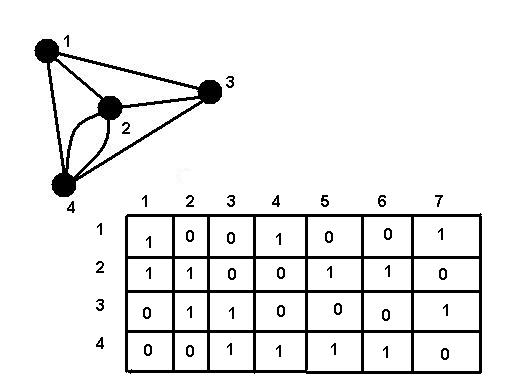
\includegraphics[width = .45\textwidth]{imagenes/Matriz_de_incidencia.JPG}

\subsection{Lista de adyacencia}
Una lista de adyacencia es un conjunto de listas ligadas donde se realiza una lista de los vecinos de cada uno de los vértices del grafo. Cada una de las listas de los vértices contiene a los vértices adyacentes.
Las listas de adyacencia ayudan a ahorrar espacio y se puede editar de manera fácil. Saber si dos vértices son adyacentes o no se vuelve más lento.
\cite{javatpoint}
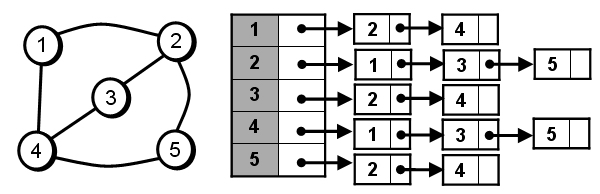
\includegraphics[width = .45\textwidth]{imagenes/Listas_de_adyacencia.jpg}


\section{Recorrido de grafos}
Los dos algoritmos utilizados para recorrer todos los nodos de un grafo son el DFS y el BFS. 
\subsection{DFS (Depth First Search)}
\begin{enumerate}
    \item Poner un vértice inicial del grafo en el tope de la pila.
    \item Poner el tope de la pila en la lista de visitados.
    \item Crear una lista de los nodos adyacentes al vértice de la lista de visitados. Agregar al tope de la pila aquellos vértices que no estén en la pila.
    \item Repetir los pasos 2 y 3 hasta que la pila esté vacía.
\end{enumerate}
\cite{dfs}
Este algoritmo es utilizado para encontrar ciclos y encontrar el camino entre dos vértices.
\subsection{BFS (Breadth-First Search)}
\begin{enumerate}
    \item Iniciar encolando el vértice inicial del grafo.
    \item Desencolar un vértice y agregarlo a la lista de visitados.
    \item Crear una lista de los nodos adyacentes al vértice de la lista de visitados. Agregar a la cola aquellos vértices que no estén en la pila.
    \item Repetir los pasos 2 y 3 hasta que la cola esté vacía.
\end{enumerate}
\cite{bfs}
Este algoritmo puede ser utilizado para encontrar los nodos vecinos de un vértice y para encontrar caminos entre dos vértices. Este algoritmo es usado en redes y en GPS. \cite{aplicaciones}

\bibliographystyle{apacite}
\bibliography{sample}

\end{document}